%-------------------------------------------------------------------------------

% This file is part of Code_Saturne, a general-purpose CFD tool.
%
% Copyright (C) 1998-2012 EDF S.A.
%
% This program is free software; you can redistribute it and/or modify it under
% the terms of the GNU General Public License as published by the Free Software
% Foundation; either version 2 of the License, or (at your option) any later
% version.
%
% This program is distributed in the hope that it will be useful, but WITHOUT
% ANY WARRANTY; without even the implied warranty of MERCHANTABILITY or FITNESS
% FOR A PARTICULAR PURPOSE.  See the GNU General Public License for more
% details.
%
% You should have received a copy of the GNU General Public License along with
% this program; if not, write to the Free Software Foundation, Inc., 51 Franklin
% Street, Fifth Floor, Boston, MA 02110-1301, USA.

%-------------------------------------------------------------------------------

\section{Solution for case4}
This case is similar to \texttt{case3}, with the following differences:

\hspace*{1cm}$\bullet\ $ \textbf{Step 1}: define head losses in the fluid domain,\\
\hspace*{1cm}$\bullet\ $ \textbf{Step 2}: compute the spatial average of temperature scalar,\\
\hspace*{1cm}$\bullet\ $ \textbf{Step 3}: parallel computation on 2 processors,\\
\hspace*{1cm}$\bullet\ $ \textbf{Step 4}: dealing with a user results file.

$\bullet$ \textbf{Step 1-1}: Define the head losses in the Graphical User Interface (GUI). \\
Go to {\itshape Volume regions definition} under the heading {\itshape Volume conditions}.
Click on {\bf``Add''}, unselect ``Initialization'' and select {\bf``Head losses''} in the box named {\itshape Nature}.
In the box named {\itshape Label}, name the head losses region. \\
Define the limits of the head losses region in {\itshape Selection criteria}.
The associated character string to enter is as below:\\
\fbox{\begin{minipage}{\textwidth}\texttt{\\
``$0.2 <= x$ and $0.4 >= x$ and $-0.75 <= y$ and $-0.25 >= y$''
}\end{minipage} }

\begin{figure}[h!]
\begin{center}
\begin{tabular}{c}
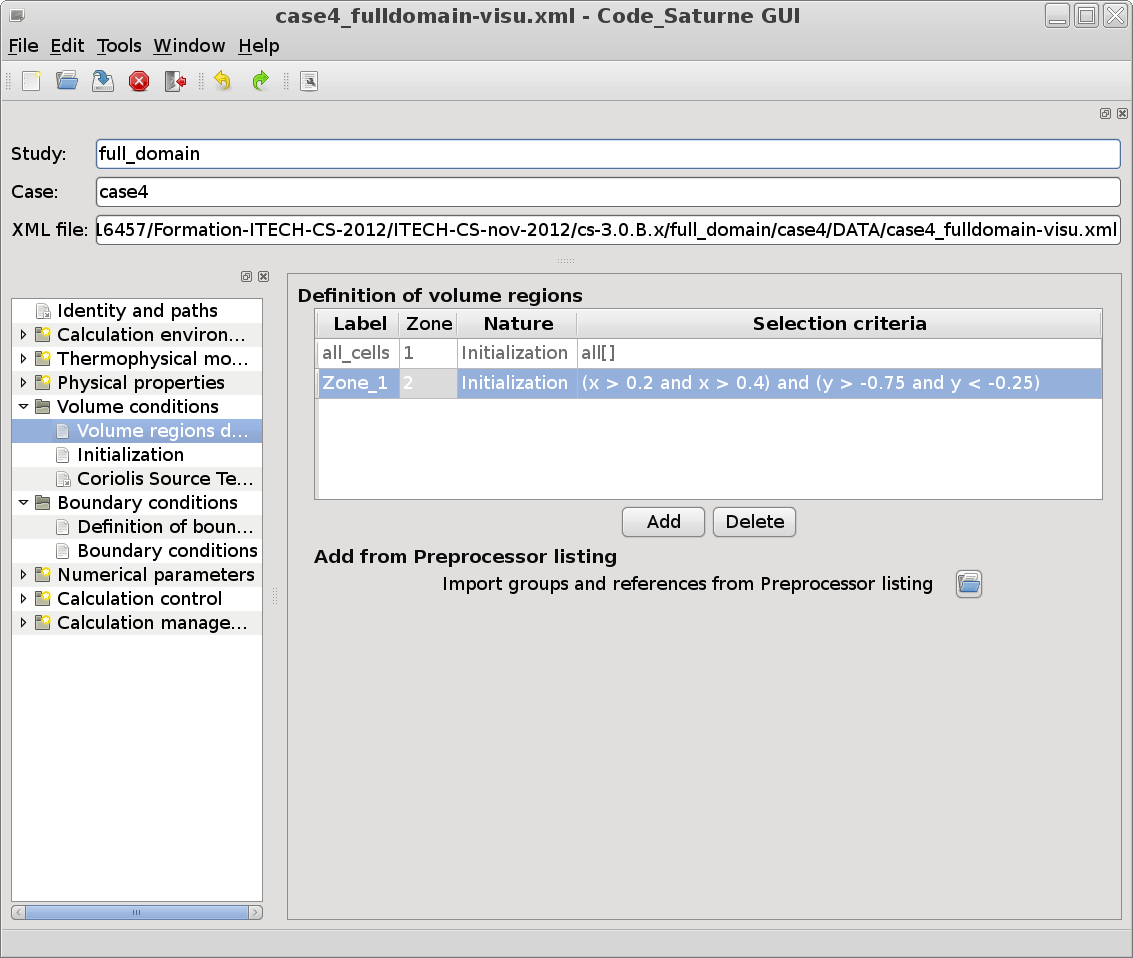
\includegraphics[width=8cm]{case4_V-1} \\
\\
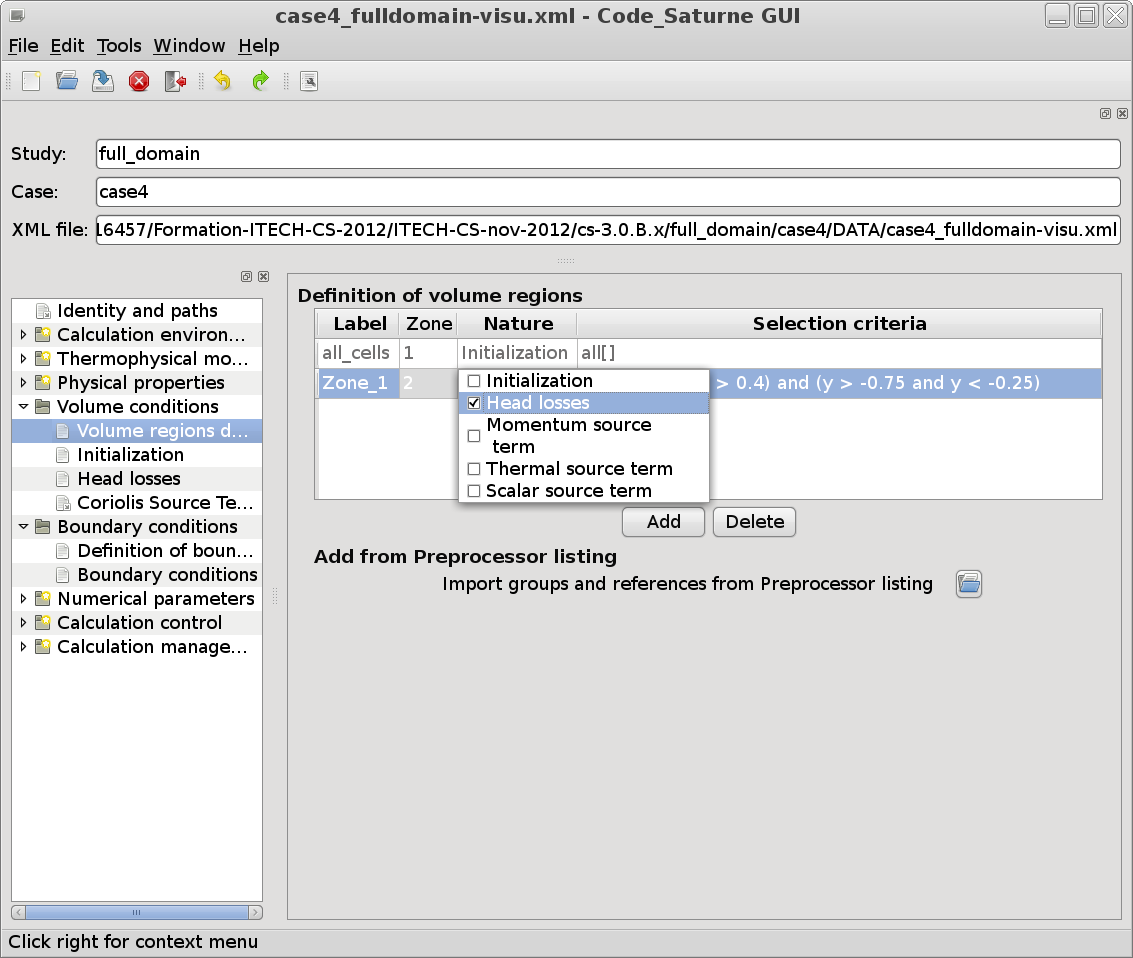
\includegraphics[width=8cm]{case4_V-2}
\end{tabular}
\caption{Creation of head losses region}
\label{fig_hl1}
\end{center}
\end{figure}

\newpage
$\bullet$ \textbf{Step 1-2}:  Specify the head losses coefficients $\alpha_{ii}$.\\
To specify the head losses coefficients go to the {\itshape Head losses} item
and select the name of the head losses volume region.
In this example, the coefficient is isotropic so that we use the same value
for each $\alpha_{ii}$. Please note that $\alpha_{ii}=2 \times K_{ii}$, therefore if
$K_{ii}=10^4$, $\alpha_{ii}=2 \ 10^4$.

\begin{figure}[h!]
\begin{center}
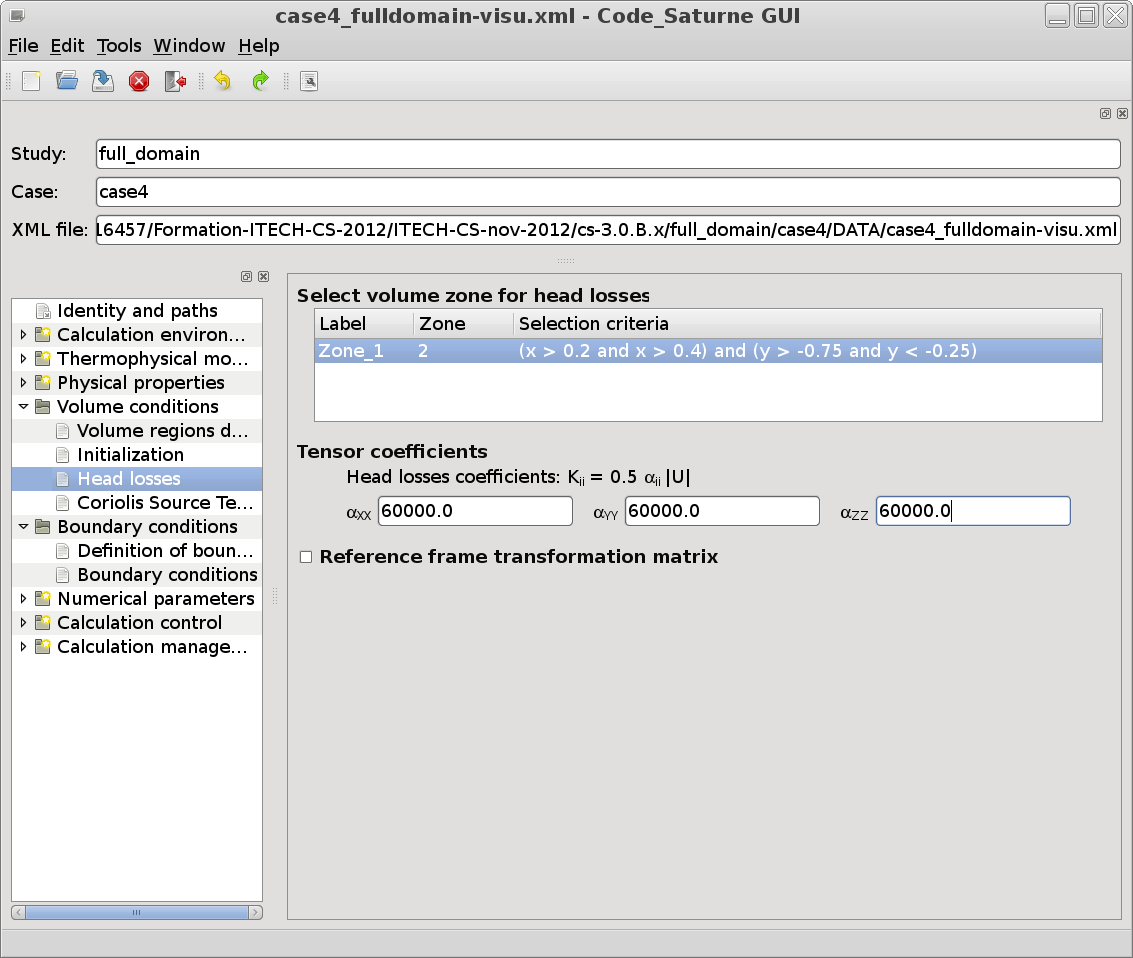
\includegraphics[width=9cm]{case4_V-3}
\caption{Head losses coefficients}
\label{fig_hl2}
\end{center}
\end{figure}

%\newpage
$\bullet$ \textbf{Step 2}:  compute the spatial average of temperature \textbf{TempC}\\
The computation of the spatial average is done in the \texttt{cs\_user\_extra\_operations.f90}
routine.\\

$\bullet$ Remark: Refer to the example files in the subdirectory \texttt{SRC/EXAMPLES} which names are:\\
\fbox{\begin{minipage}{\textwidth}\texttt{                  \\
 cs\_user\_extra\_operations-energy\_balance.f90            \\
 cs\_user\_extra\_operations-extract\_1d\_profile.f90       \\
 cs\_user\_extra\_operations-force\_temperature.f90         \\
 cs\_user\_extra\_operations-global\_efforts.f90            \\
 cs\_user\_extra\_operations-parallel\_operations.f90       \\
 cs\_user\_extra\_operations-print\_statistical\_moment.f90
}\end{minipage} }

To correctly complet your \texttt{cs\_user\_extra\_operations.f90} routine
(copied in the \texttt{SRC} directory), you can use mainly these examples files:
\texttt{cs\_user\_extra\_operations-print\_statistical\_moment.f90} and
\texttt{cs\_user\_extra\_operations-extract\_1d\_profile.f90}.

$\bullet$ \textbf{Step 3}: choose a computation with 2 processors \\
This modification will be done in the {\itshape Prepare batch analysis} item.\\
To run the calculation on two processors, simply change the number of processors
indicator to 2. The launch script will automatically deal with the rest.

\begin{figure}[h!]
\begin{center}
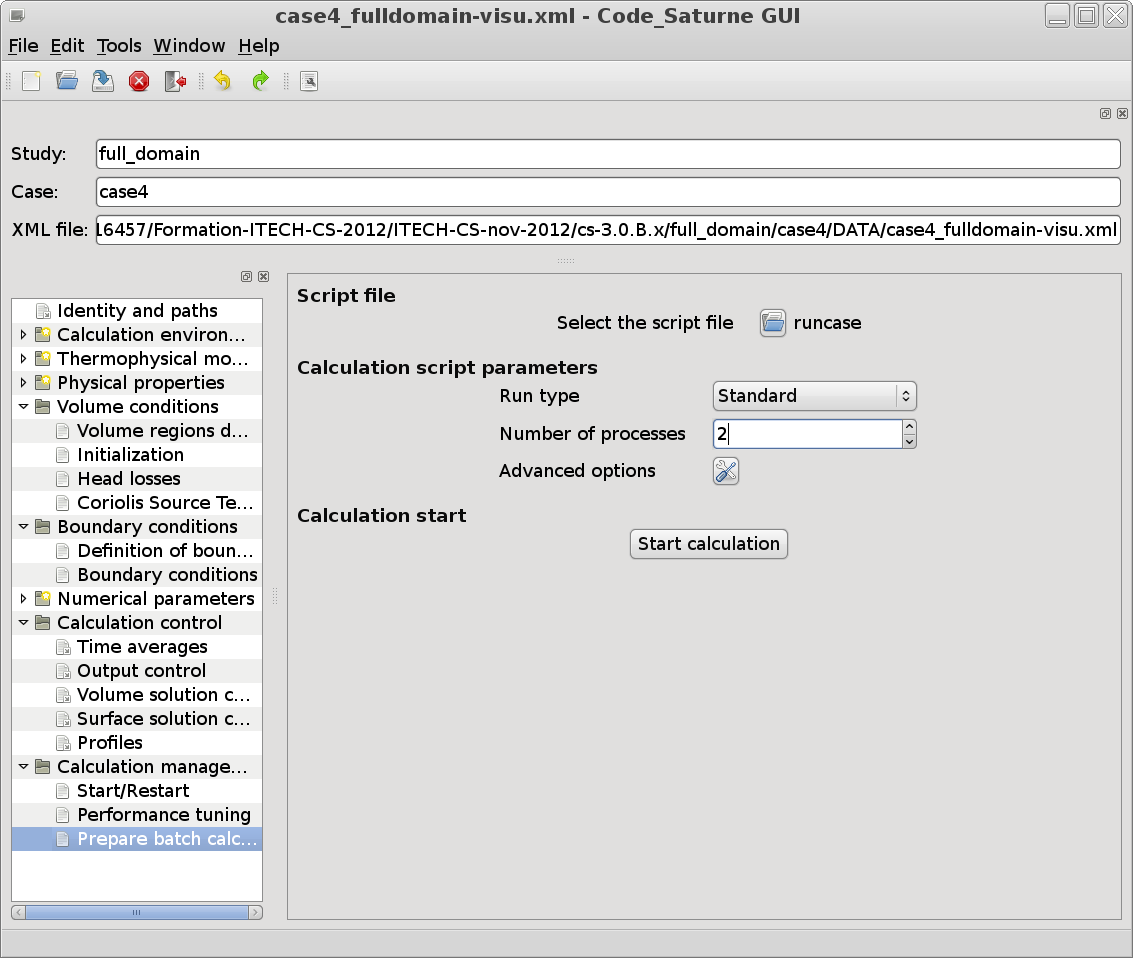
\includegraphics[width=9cm]{case4_V-4} % 12cm
\caption{Number of processors}
\label{fig1_e4}
\end{center}
\end{figure}

\newpage
$\bullet$ \textbf{Step 4}:  dealing with a user results file \textbf{``moy.dat''}\\
The new user file ``moy.dat'' created by \texttt{cs\_user\_extra\_operations.f90}
will be written directly in the \texttt{yyyymmdd-hhmm} results subdirectory created
at the end of the computation in the \texttt{RESU} directory.

$\bullet$ Remark : We do not have to specify the name of the new user file in the
Graphical User Interface (GUI), like in previous \CS versions. \\
The name of the new user file had to be identified in the launch script in order
to be automatically copied in the \texttt{RESU} directory, this is not requested.

\begin{figure}[h!]
\begin{center}
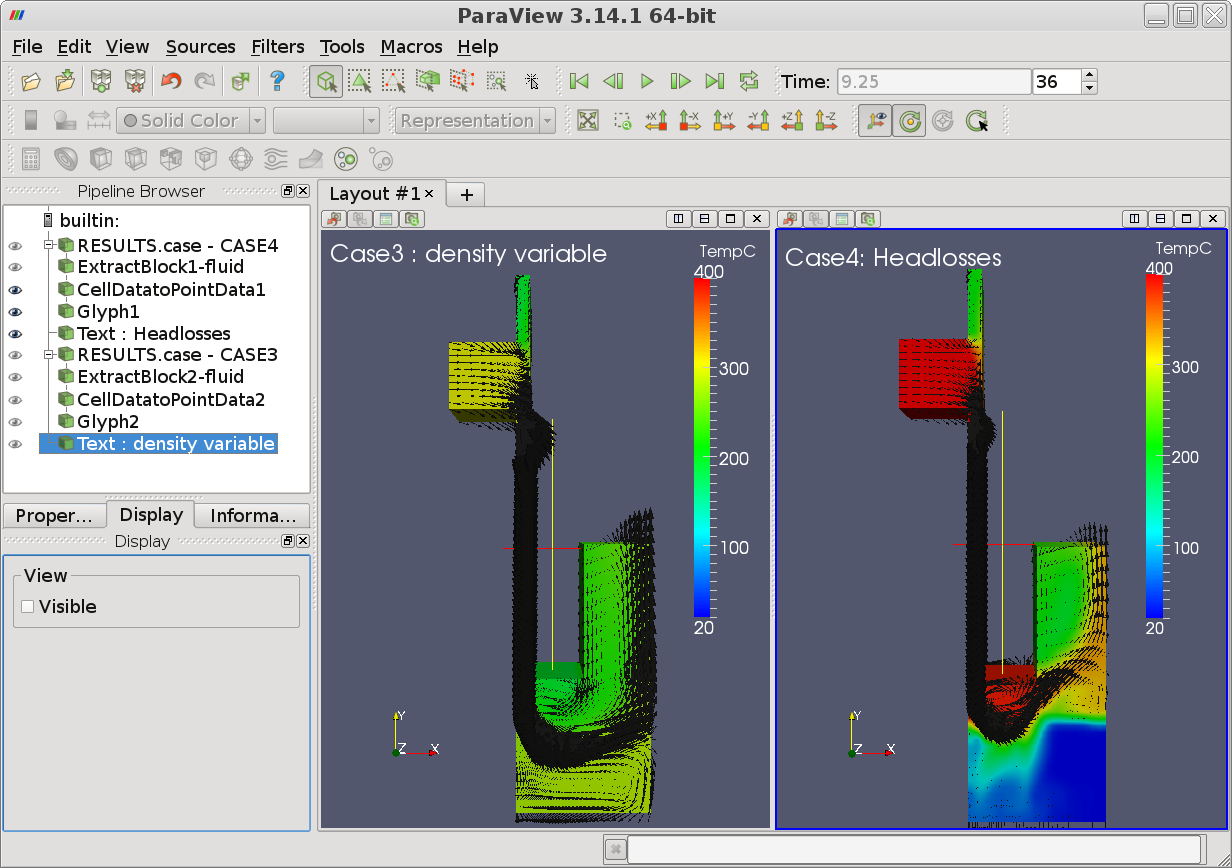
\includegraphics[width=11cm]{case4_V-5-paraview}
\caption{User results files}
\label{fig2_e4}
\end{center}
\end{figure}


